\documentclass[11pt,a4paper]{article}

% Standard packages only: this file compiles with a stock TeX Live, with
% `tectonic main.tex`, or on arXiv, and it needs no shell escape.
\usepackage[T1]{fontenc}
\usepackage[utf8]{inputenc}
\usepackage{lmodern}
\usepackage[margin=1in]{geometry}
\usepackage{booktabs}
\usepackage{amsmath}
\usepackage{graphicx}
\usepackage{microtype}
\usepackage{tikz}
\usetikzlibrary{arrows.meta,positioning}
\usepackage[colorlinks=true,allcolors=blue]{hyperref}

\title{\textbf{SiteSurveyor}: A Hybrid On-Chain/Off-Chain Workspace\\
for Survey Operations, Evidence Provenance, and Settlement}

\author{Consolation Mangena\\
Eineva Labs\\
\href{https://sitesurveyor.tech}{sitesurveyor.tech}}

\date{November 2026}

\begin{document}
\maketitle

\begin{abstract}
Field survey work is usually split across a paper field book, a spreadsheet, a file
share and several disconnected business systems. Every hand-off loses context, and
evidence gathered in the field is rarely bound to the record it is supposed to
support. This paper describes \textbf{SiteSurveyor}, an open-source, multi-tenant
workspace that keeps the operational record --- project, job, quote, invoice,
evidence and payment --- continuous, while keeping confidential survey content
off-chain. The system combines a React/TypeScript progressive web app, a PostgreSQL
backend with row-level security, and a small set of edge functions. Solana is used
only where it adds a property the database cannot supply: wallet-based sign-in,
stablecoin settlement, and a wallet-signed digest that lets a third party confirm
that a file presented later is byte-identical to the one that was anchored. An AI
agent operates the same records through an allowlisted tool surface, with read-back
verification of writes and explicit confirmation before destructive actions. We
report the design, the security boundaries, and the engineering evidence behind the
current release, and we are explicit about what a file digest does \emph{not} prove.
\end{abstract}

\section{Introduction}

A survey engagement produces more than coordinates. It produces a quote, a schedule,
a crew assignment, field observations, photographs, CAD drawings, cost records, an
invoice and, eventually, a payment. In common practice these artefacts live in
different tools: a field book or a phone note for observations, a spreadsheet for
pricing, a shared drive for photographs, and an accounting package for the invoice.
The project identifier is the only thing that connects them, and it is re-entered by
hand at every boundary.

Two problems follow. The first is \emph{operational}: the state of a job is
reconstructed from several partial views, and the reconstruction is frequently
stale. The second is \emph{evidential}: a file handed to a client or a regulator
later cannot easily be shown to be the file that was produced in the field. Both
problems are usually addressed by buying more software, which adds further
boundaries rather than removing them.

SiteSurveyor takes the opposite approach: one workspace holds the continuous record,
and external systems are used only for properties the workspace itself cannot
provide. The contributions described here are:

\begin{enumerate}
  \item a data model that binds quote, project, job, evidence, cost and payment to a
        single tenant-scoped record, enforced by PostgreSQL row-level security
        rather than by application code alone;
  \item an evidence-integrity mechanism with two modes --- a hash-only anchor that
        publishes nothing but an attachment identifier and a SHA-256 digest, and an
        opt-in encrypted full-file mode whose ciphertext never leaves storage;
  \item an AI agent that is treated as an \emph{operational} actor: it calls a typed,
        allowlisted tool surface, reads its own writes back before reporting success,
        and requires explicit confirmation for destructive operations;
  \item a satellite analysis engine that turns open Earth-observation products into
        ranked field targets and deliverables the workspace can render;
  \item a deployment and verification story that is honest about its limits,
        including which components remain sandboxed or unimplemented.
\end{enumerate}

The remainder of the paper describes the requirements (Section~\ref{sec:req}), the
architecture (Section~\ref{sec:arch}), the data and identity model
(Section~\ref{sec:data}), the agent (Section~\ref{sec:agent}), evidence anchoring
(Section~\ref{sec:evidence}), the security model (Section~\ref{sec:security}), the
Earth-observation engine (Section~\ref{sec:eo}), the engineering evidence
(Section~\ref{sec:eval}), and the limitations (Section~\ref{sec:limits}).

\section{Requirements}
\label{sec:req}

The design is driven by five constraints observed in small and mid-sized surveying
practices.

\begin{description}
  \item[Confidentiality.] Client identities, coordinates, valuations and drawings are
        commercially sensitive. They must not be published to a public ledger, and
        they must not be sent to a model provider unless a user explicitly supplies
        them.
  \item[Continuity.] A record created in one stage must remain attached to the same
        project in every later stage, including after a device change.
  \item[Verifiability.] It must be possible to show, later and to a third party, that
        a presented file is the file that was recorded --- without revealing the file
        to that third party.
  \item[Field use.] The interface has to work on a phone in daylight, survive poor
        connectivity, and remain keyboard-operable in the office.
  \item[Honest state.] Sandbox payments, development clusters and unimplemented
        surfaces must be visibly distinguishable from production behaviour. A demo
        that looks settled when nothing settled is worse than no demo.
\end{description}

\section{Architecture}
\label{sec:arch}

The implemented system is a responsive React single-page application, installable as
a progressive web app, backed by Supabase \cite{supabase} (PostgreSQL, Storage, Auth
and edge functions) with Solana \cite{yakovenko2017} for identity, settlement and file
digests. A Tauri \cite{tauri} (Rust) shell packages the same frontend as a desktop
window. The architecture is
\emph{hybrid by default}: operational and confidential data stay in the database,
and the chain carries only explicit transactions and a minimal digest statement.

\begin{figure}[t]
\centering
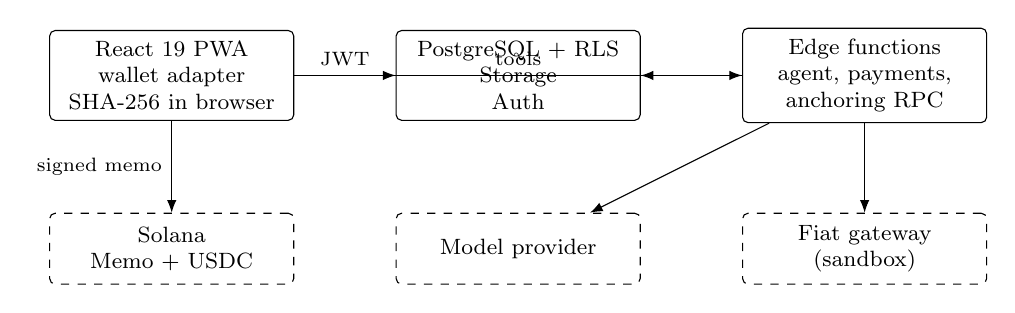
\begin{tikzpicture}[
  font=\footnotesize,
  box/.style={draw, rounded corners=2pt, align=center, inner sep=4pt,
              minimum height=9mm, minimum width=3.1cm},
  ext/.style={draw, dashed, rounded corners=2pt, align=center, inner sep=4pt,
              minimum height=9mm, minimum width=3.1cm},
  ar/.style={-{Latex[length=1.6mm]}, thin}
]
  \node[box] (ui) at (0,0) {React 19 PWA\\wallet adapter\\SHA-256 in browser};
  \node[box] (db) at (4.4,0) {PostgreSQL + RLS\\Storage\\Auth};
  \node[box] (fn) at (8.8,0) {Edge functions\\agent, payments,\\anchoring RPC};

  \node[ext] (sol) at (0,-2.2) {Solana\\Memo + USDC};
  \node[ext] (nim) at (4.4,-2.2) {Model provider};
  \node[ext] (fiat) at (8.8,-2.2) {Fiat gateway\\(sandbox)};

  \draw[ar] (ui) -- node[above]{\scriptsize JWT} (db);
  \draw[ar] (ui) -- node[above]{\scriptsize tools} (fn);
  \draw[ar] (fn) -- (db);
  \draw[ar] (ui) -- node[left]{\scriptsize signed memo} (sol);
  \draw[ar] (fn) -- (nim);
  \draw[ar] (fn) -- (fiat);
\end{tikzpicture}
\caption{Trust boundaries. Confidential records never leave the database boundary
except as explicitly supplied context; the chain receives only an attachment
identifier and a digest, or a user-signed transfer.}
\label{fig:arch}
\end{figure}

\begin{table}[t]
\centering
\caption{Deployed components and responsibilities.}
\label{tab:components}
\small
\begin{tabular}{@{}p{0.22\linewidth}p{0.70\linewidth}@{}}
\toprule
Component & Responsibility \\
\midrule
Web app & Workspaces, projects, jobs, files, finance, market, Earth-observation views \\
Desktop shell & Tauri v2 window over the same bundle; off-origin navigation is handed to the system browser \\
Edge functions & Agent endpoint, RPC proxy, fiat operations, wallet nonces, anchoring metadata, job dispatch \\
Satellite engine & Python worker that claims survey runs, runs raster pipelines and publishes deliverables \\
MCP server & The same screening surface exposed over the Model Context Protocol \\
AI gateway & Optional self-hosted alternate host for the agent contract \\
\bottomrule
\end{tabular}
\end{table}

Three deployment shapes are supported from the same source: a static host that
publishes the built bundle, a multi-stage container image served by Nginx, and the
optional Node gateway that additionally serves the agent endpoint. Build-time
variables become browser configuration, which is why no server secret may be supplied
through them; the repository documents this boundary and a secret scan enforces it.

\section{Data, identity and tenancy}
\label{sec:data}

\paragraph{Schema as source of truth.}
The database is described by 63 ordered migrations. The first is a dump of the
deployed schema; the rest are incremental. Together they rebuild an empty database
into the current state, and the generated TypeScript types are checked so that the
client cannot drift from the SQL.

\paragraph{Workspaces.}
An account belongs to one or more workspaces: a \emph{personal} workspace for an
independent professional, a \emph{business} workspace for a firm with dispatch and
staff, and a \emph{platform operator} view for administration. Row-level security
\cite{pg-rls} policies key on workspace membership, so the same tables serve all three
shells and authorisation does not depend on which screen the client happens to render.

\paragraph{Identity.}
Email and GitHub sign-in are supported alongside Sign In With Solana, where the user
signs a random nonce with a wallet \cite{walletstandard}. Sessions are held by the Supabase client;
restoration from a cached session is treated as presentation only and never as
evidence that a remote operation succeeded. The desktop build cannot receive OAuth
redirects directly, so a bridge page on the web origin forwards the callback to a
registered application protocol; the PKCE verifier then completes the exchange
exactly as it would in a browser.

\section{The agent as an operational actor}
\label{sec:agent}

The assistant is not a chat window bolted onto the product. A user's bearer token is
sent to an edge function that authenticates the caller, checks conversation
ownership, resolves the workspace, runs a shared agent core and streams events as
newline-delimited JSON (\texttt{status}, \texttt{tool}, \texttt{delta},
\texttt{final}, \texttt{error}). A self-hosted Node gateway implements the same
contract, and an MCP server mirrors the tool surface so an external MCP host can use
it \cite{mcp}.

The controls that make this safe are structural rather than prompt-based:

\begin{itemize}
  \item models are restricted by a shared allowlist, so a request cannot select an
        arbitrary provider model;
  \item reads and writes are restricted to allowlisted tables, and the live schema is
        supplied so the model uses real columns;
  \item write payloads are validated against the schema, and new business records are
        stamped with the resolved workspace rather than a model-supplied one;
  \item insert and update results are read back and marked verified before the agent
        is allowed to report success;
  \item updates and deletes require a valid UUID, and a permanent delete additionally
        requires an explicit confirmation flag;
  \item identical repeated calls and the total number of tool rounds are capped;
  \item conversation history is bounded with summarisation and optional structured
        memory.
\end{itemize}

CAD operations are deliberately read-only in the tool surface: the agent can inspect
drawings, layers and entity counts, but geometry changes are emitted as command blocks
that the user executes in the project workspace, with an extra confirmation for
erasing. This keeps a generative component away from the authoritative drawing.

\section{Evidence integrity and anchoring}
\label{sec:evidence}

Files are uploaded to object storage and described in the database. The browser
computes a lowercase hex SHA-256 \cite{fips180} with the Web Crypto API. Verification
re-downloads the object, recomputes the digest and compares it with the recorded
value.

Two anchoring modes are implemented. In \emph{hash-only} mode --- the default ---
only the attachment identifier and digest are written to a Solana Memo instruction:

\begin{verbatim}
ssv1:<attachment-id>:sha256:<file-hash>
ssv2:<attachment-id>:sha256:<file-hash>:<manifest-hash>:<chunk-count>
\end{verbatim}

Because the identifier is an opaque UUID, a reader can associate the proof with an
attachment without learning anything about its contents or its owner. In the opt-in
\emph{full-file} mode the plaintext is encrypted with AES-256-GCM
\cite{sp800-38d} under a key derived by PBKDF2-SHA256 \cite{rfc8018} from a
user-supplied passphrase, split into ordered 256\,KiB chunks
with per-chunk digests, and stored with a manifest under
\texttt{<workspace-id>/anchors/<operation-id>/}. The chain receives the manifest hash
and chunk count, never the chunk digests and never the file. Recovery downloads,
decrypts, re-hashes and reassembles, so key custody remains with the user: losing the
passphrase costs the redundant chunk copies, not the original.

Transactions are signed and fee-paid by the connected wallet, and the recorded
signature, slot and fee make the anchor auditable. A digest proves byte equivalence
at a point in time. It does not prove authorship, ownership, survey accuracy or legal
validity, and the product copy says so wherever an anchor is shown.

\begin{table}[t]
\centering
\caption{What an anchored digest does and does not establish.}
\label{tab:proves}
\small
\begin{tabular}{@{}ll@{}}
\toprule
Established & Not established \\
\midrule
The presented bytes equal the digested bytes & Who produced the bytes \\
The digest existed on-chain at a slot & That the survey is correct \\
The wallet paid for and signed the statement & Legal ownership or title \\
The manifest identifies the chunk set & Confidentiality of the plaintext \\
\bottomrule
\end{tabular}
\end{table}

\section{Security model}
\label{sec:security}

\paragraph{Data classification.}
Table~\ref{tab:classification} is maintained as part of the design, and new tools must
update it. It is the document a reviewer reads before enabling a deployment, because
it states where each class of data is allowed to appear.

\begin{table}[t]
\centering
\caption{Data classification by store. ``Supplied'' means only when a user explicitly
includes it in a request.}
\label{tab:classification}
\footnotesize
\begin{tabular}{@{}p{0.27\linewidth}cccp{0.30\linewidth}@{}}
\toprule
Data & Postgres & Storage & AI & Chain \\
\midrule
Profile and workspace & yes & no & context & address may be public \\
Operational records & yes & no & tool context & no \\
Original survey files & metadata & yes & supplied only & no \\
File digest and id & yes & no & supplied only & yes, on anchor \\
Conversations and memory & yes & no & prompt/history & no \\
Payment records & yes & no & supplied only & transfers only \\
\bottomrule
\end{tabular}
\end{table}

\paragraph{Privileged functions are closed.}
Maintenance jobs write through a service-role client, because their rows belong to
other tenants. A job that is merely ``authenticated'' is therefore a cross-tenant
write primitive. The backfill function now requires the project's service key and
compares it against the configured secret in constant time; it does not inspect a
JWT claim, because an unverified \texttt{role} claim is attacker-controlled and would
otherwise let any caller forge a service token. Tests cover valid, invalid and forged
credentials.

\paragraph{Enumeration.}
The pre-authentication email check needs to answer ``is this address already
registered''. Left uncapped it is an enumeration oracle, so the lookup is rate-limited
in the database rather than in the client, where a limit could be bypassed.

\paragraph{Secrets.}
Only public configuration is compiled into the bundle. Server secrets live in the
function and engine environments. Continuous integration runs a pinned secret scanner
over the full history on every push and weekly, with a narrowly scoped allowlist for
values that are public by design, such as publishable API keys.

\paragraph{Non-claims.}
The repository states plainly what the system does not do: it does not certify
accuracy, it does not make a sandbox payment settled, and it does not treat a hash as
proof of authorship. Reviewers of a deployment are given a checklist covering row
level security, storage policies, function authorisation, cluster consistency and
payment reconciliation.

\section{Earth-observation engine}
\label{sec:eo}

Survey screening is a Python worker rather than a browser feature. It ingests
multi-sensor open data --- Sentinel-2 surface reflectance \cite{drusch2012}, a 30\,m
Copernicus digital elevation model, ALOS PALSAR radar, Landsat water observations
\cite{mueller2016}, ESA WorldCover and CHIRPS rainfall \cite{funk2015} --- onto a common
30\,m grid in UTM~35S, and runs four category pipelines: groundwater potential with
candidate borehole sites, mineral prospectivity with ranked targets, soil capability
with erosion risk, and multi-hazard risk with safest buildable sites. Weights come from
an analytic hierarchy process \cite{saaty1980} over the available indices, and
deliverables are published as GeoTIFF, GeoJSON, CSV, KMZ and a PMTiles archive for the
map workbench. Imagery is acquired from the Digital Earth Africa open data cube
\cite{dea}.

The worker claims rows with \texttt{FOR UPDATE SKIP LOCKED}, so several workers can
run safely, and it never touches authentication, sessions or wallets. The same
pipelines are exposed over the Model Context Protocol, which is what allows an MCP
host to run the identical screening outside the platform.

This component analyses imagery; it does not store evidence. Anchoring and Earth
observation are deliberately separate features, because conflating ``we can compute a
map'' with ``we can prove a file'' would overstate both.

\section{Engineering evidence}
\label{sec:eval}

The claim that the described system exists is supported by continuous checks rather
than by demonstration alone:

\begin{itemize}
  \item TypeScript project checks and a strict lint pass over the web application;
  \item more than 850 automated TypeScript tests and 124 edge-function tests,
        including the service-key gate, the payment state machine and the anchoring
        state machine;
  \item a production build, which also generates the sitemap and copies the security
        contact file;
  \item deterministic evaluation scripts for the agent: tool-shape consistency,
        memory behaviour, model allowlists and round budgets;
  \item workflow linting, and a secret scan over the entire commit history.
\end{itemize}

These are engineering checks, not a user study. No claim is made here about
productivity, accuracy of the geospatial screening against ground truth, or usability
measured with practitioners; those are the obvious next evaluations and are named as
such rather than implied by a demo.

\section{Limitations and threats to validity}
\label{sec:limits}

\begin{itemize}
  \item \textbf{A digest is not provenance.} The anchor binds bytes to a wallet and a
        slot. Identity behind the wallet, authorship and correctness remain social and
        legal questions.
  \item \textbf{Model behaviour is bounded, not proved.} Allowlists, schema validation
        and read-back verification reduce the failure surface; they do not guarantee
        that every agent statement is true, which is why writes are verified and
        deletes confirmed.
  \item \textbf{Sandbox defaults.} Committed defaults point at a development cluster
        and a sandbox fiat gateway. Production settlement is an explicit deployment
        decision, and the interface distinguishes pending, sandbox and settled states.
  \item \textbf{Policy is the perimeter.} Tenant isolation rests on row-level security.
        A missing or wrong policy is a vulnerability; the deployment checklist and
        tests target this class of error but cannot prove its absence.
  \item \textbf{Incomplete surfaces.} The mobile shell is a placeholder, and some
        marketplace data is synthetic. The interface labels each of these.
  \item \textbf{Single-region demonstration.} The public deployment is a reference
        implementation, not a multi-region service with measured availability.
\end{itemize}

\section{Availability and reproducibility}
\label{sec:availability}

\begin{sloppypar}
The implementation is released under the MIT licence at
\url{https://github.com/ConsoleMangena/sitesurveyor-framework}. Releases are archived
on Zenodo, which mints a version DOI under a stable concept DOI, and the repository
carries citation metadata so that a release can be cited without consulting this
paper. The repository does not ship a shared hosted instance: an adopter supplies
their own database project, Earth-observation token and provider keys, and the
documentation states which configuration values are public.
\end{sloppypar}

Building the paper requires only a standard \LaTeX{} installation; the source and
bibliography are in the \texttt{paper/} directory of the repository.

\section{Conclusion}

Survey operations are not short of software; they are short of continuity. Keeping
the operational record in one tenant-scoped workspace removes the re-entry boundaries
that lose context, and reserving the chain for wallet identity, settlement and a
minimal digest keeps confidential content where it belongs. The same architecture
treats an AI agent as an actor with a narrow tool contract and verified writes rather
than as an oracle, and it states its limitations where a user will read them. The
next steps are external evaluation of the screening against field data and a
practitioner study of the workspace itself.

\bibliographystyle{plain}
\bibliography{references}

\end{document}
